\chapter{Equalizer GPU Implementation and Bit Error Rate Performance}
\label{chap:equalizers_in_gpus}
\section{GPU Implementation}
Each equalizer in the PAQ system presents an interesting challenge from a GPU implementation perspective.
The equations for each equalizer were presented in Section \ref{sec:equalizer_eq}.
In this chapter, the equalizer equations are reformulated for fast and efficient GPU implementation, 

Every equalizer filter is computed using batch processing.
In batch processing, each packet is independent of all other packets.
Each packet in a batch is processed in exactly the same way with different data.
To simplify the figures, every block diagram in this chapter shows how one packet is processed.
The processing is repeated $3104$ times to compute a full batch of equalizer filters.

Convolution is used many times in this chapter.
Section \ref{sec:batched_convolution} showed that GPU frequency-domain convolution using batch processing performs best for the PAQ system.
To simplify block diagrams, frequency-domain convolution is shown as one block, as illustrated in
Figures \ref{fig:Conv2} and \ref{fig:Conv3}.

Note that the detection filter $\mathbf{d}$ and the SOQPSK-TG power spectral density $\mathbf{\Psi}$ are defined constants.
The SOQPSK-TG power spectral density $\mathbf{\Psi}$ and $\mathbf{D}$, the $16$,$384$-point FFT of $\mathbf{d}$, are precomputed and stored.
Applying $\mathbf{d}$ in the frequency domain does not require an extra FFT, only extra complex multiplies.
\begin{figure}
	\centering\includegraphics[width=7.73in/100*55]{figures/eq_GPUimplementation/Conv2.pdf}
	\caption{A block diagram representation of $\mathbf{y} = \mathbf{x} * \mathbf{c}$.
			 Convolution is performed in the frequency domain.
			 All the required operations in the top part of the figure are represented by the block in the lower part of the figure.}
	\label{fig:Conv2}
\end{figure}
\begin{figure}
	\centering\includegraphics[width=7.78in/100*55]{figures/eq_GPUimplementation/Conv3.pdf}
	\caption{A block diagram representation of $\mathbf{y} = (\mathbf{x} * \mathbf{c} ) * \mathbf{D}$ (cascaded convolution), where $\mathbf{D}$ is the FFT of a filter that does not change with the data (i.e. $\mathbf{D}$ is precomputed and stored.
	Convolution is performed in the frequency domain.
	All the required operations in the top part of the figure are represented by the block in the lower part of the figure.}
	\label{fig:Conv3}
\end{figure}

\clearpage
\subsection{Zero-forcing and MMSE GPU Implementation}
The ZF and MMSE FIR equalizer filter coefficient computations have exactly the same form as shown in Equations \eqref{eq:start_here_ZF_MDR} and \eqref{eq:start_here_MMSE_MDR}.
Consequently any algorithm reconstructing that improves the efficiency of computing the MMSE equalizer coefficients, also applies to computing the ZF filter coefficients.
Three approaches to computing the equalizer filter coefficients were explored:
\begin{itemize}
\item Using the Levinson-Durbin recursion algorithm to solve $\mathbf{R} \mathbf{c}_\text{MMSE} = \hat{\mathbf{g}}$ leveraging the toeplitz property of $\mathbf{R}$.
\item Using the cuBLAS LU decomposition library to compute the inverse and matrix vector multiplication defined by $\mathbf{c}_\text{MMSE} = \mathbf{R}^{-1} \hat{\mathbf{g}}$.
\item Using the cuSolver library to solve $\mathbf{R} \mathbf{c}_\text{MMSE} = \hat{\mathbf{g}}$ by leveraging the sparse property of $\mathbf{R}$.
\end{itemize}
For reference, the matrix $\mathbf{R}$ is
\begin{equation}
\mathbf{R} = 
		\begin{bmatrix}
		r_{\hat{h}}(0) + \hat{\sigma}^2_w			& r^\ast_{\hat{h}}(1)	& \cdots 	& r^\ast_{\hat{h}}(L_{eq}-1)  	\\
		r_{\hat{h}}(1) 			& r_{\hat{h}}(0) + \hat{\sigma}^2_w		& \cdots 	& r^\ast_{\hat{h}}(L_{eq}-2)  	\\
		\vdots	 				& \vdots				& \ddots 	&  								\\
		r_{\hat{h}}(L_{eq}-1)	& r_{\hat{h}}(L_{eq}-2)	& \cdots	& r_{\hat{h}}(0) + \hat{\sigma}^2_w  			
	\end{bmatrix}.
	\label{eq:R_h_ref}
\end{equation}

The Levinson-Durbin recursion algorithm avoids the $\mathcal{O}(n^3)$ operations normally associated with solvers by leveraging the Toeplitz or diagonal-constant structure of $\mathbf{R}$ \cite[Chap. 5]{hayes:1996}.
The first GPU implementation of the Levinson-Durbin recursion algorithm computed the MMSE equalizer filter assuming the matrix $\mathbf{R}$ and the vector $\hat{\mathbf{g}}$ were real-valued.
The Levinson-Durbin recursion algorithm showed promise by computing $3104$ real-valued MMSE equalizer filters in $500$ ms.
The GPU implementation of Levinson-Durbin recursion was then converted to the complex-valued case.
The Levinson-Durbin recursion computed $3104$ complex-valued MMSE equalizer filters in $2$,$500$ ms, in excess of the $1907$ ms maximum for all processing time.

The next algorithm explored computed the inverse of $\mathbf{R}$ using the cuBLAS batch processing library.
The cuBLAS library computes a \textit{complex-valued} inverse using the LU decomposition in $600$ ms.
cuBLAS executed faster than the Levinson-Durbin recursion algorithm, but $600$ ms is still $31\%$ of the total $1907$ ms processing time.

The final and fastest algorithm explored solves $\mathbf{c}_\text{MMSE} = \mathbf{R}^{-1} \hat{\mathbf{g}}$ by leveraging the sparse properties of $\mathbf{R}$ using the cuSolverSp batch processing library.
The $ 186 \times 186)$ auto-correlation matrix $\mathbf{R}$ comprises the sample auto-correlation $r_{\hat{h}}(k)$ and the noise variance estimate $\hat{\sigma}^2_w$.
Because the sample auto-correlation $r_{\hat{h}}(k)$ only has support on $-37 \leq k \leq 37$ and the addition of $\hat{\sigma}^2_w$ does not increase that support, the auto-correlation matrix $\mathbf{R}$ is sparse: $63\%$ of its entries are zeroes.
``cusolverSpCcsrqrsvBatched'' is the GPU function used from the cuSolverSp library.
cusolverSpCcsrqrsvBatched is a complex-valued solver that leverages batch processing and the sparse properties of $\mathbf{R}$ by exploiting Compressed Row Storage (CRS) \cite{wiki:Sparse_matrix}.
CRS reduces the large $186\times186$ matrix to a $12544$ element CSR matrix $\mathbf{R}_{\text{CRS}}$.
Before cusolverSpCcsrqrsvBatched can be called, the CSR matrix $\mathbf{R}_{\text{CRS}}$ has to be built and the vector $\hat{\mathbf{g}}$ has to be built.
An example of how to use the CUDA cusolverSp library can be found in \cite{CUDA_toolkit_doc}.

Figures \ref{fig:blockZF} and \ref{fig:blockMMSE} show how the ZF and MMSE equalizer filters are computed and applied to the received samples, respectively.
Note that the equalizer filters are applied in the frequency-domain with the detection filter.
\begin{figure}
	\centering\includegraphics[width=10.51in/100*55]{figures/eq_GPUimplementation/blockZF.pdf}
	\caption{Block diagram showing how the zero-forcing equalizer coefficients are implemented in the GPU.}
	\label{fig:blockZF}
\end{figure}
\begin{figure}
	\centering\includegraphics[width=10.64in/100*55]{figures/eq_GPUimplementation/blockMMSE.pdf}
	\caption{Block diagram showing how the minimum mean-squared error equalizer coefficients are implemented in the GPU.}
	\label{fig:blockMMSE}
\end{figure}
Table \ref{tab:ZFMMSEtimingComparison} lists the algorithms researched and their respective execution times.
\begin{table}
\caption{Algorithms used to compute the ZF and MMSE equalizer filters.}
\begin{center}
\begin{tabular}{lll}
	\toprule
	Algorithm 			& Data type	& Execution Time (ms)	\\ \midrule
	Levinson Recursion 	& Real	 	& 500 					\\
	Levinson Recursion 	& Complex 	& 2500 					\\
	LU Decomposition 	& Complex 	& 600				 	\\
	cuSolver			& Complex	& 356				\\
	\bottomrule
\end{tabular}
\end{center}
\label{tab:ZFMMSEtimingComparison}
\end{table}

\subsection{Constant Modulus Algorithm GPU Implementation}
The CMA equalizer is an adaptive FIR filter, where the filter coefficients are updated on a packet-by-packet basis using a steepest descent algorithm shown in Equation \eqref{eq:steepest}.
The more iterations the steepest descent algorithm executes, the more effective the CMA equalizer is.
The most computationally heavy operation in the CMA update is computing $\nabla J$, shown in Equation \eqref{eq:DelJcma-approxr_MDR} and repeated here for reference
\begin{equation}
	\nabla J = \frac{2}{L_{pkt}} \sum_{n=0}^{L_{pkt}-1}
	\left[ \vphantom{\displaystyle\sum}  \hat{s}^{(b)}(n) \left( \hat{s}^{(b)}(n)\right)^\ast - 1 \right]
	\hat{s}^{(b)}(n)  \tilde{\mathbf{r}}^\ast(n),
\label{eq:DelJcma-approxr_ref}
\end{equation}
where $\tilde{\mathbf{r}}^\ast(n)$ is defined in \eqref{eq:r_tilde_n}.
Two approaches to computing the equalizer filter coefficients were explored:
\begin{itemize}
\item Computing $\nabla J$ directly using the summation in Equation \eqref{eq:DelJcma-approxr_ref}.
\item Reformulating $\nabla J$ into convolution to leverage the fast computation time of convolution using batch processing in GPUs.
\end{itemize}
To simplify the analysis of each option, \eqref{eq:DelJcma-approxr_ref} is expressed as
\begin{equation}
	\nabla J = \frac{1}{L_\text{pkt}} \sum_{n=0}^{L_\text{pkt}-1}
	z(n)  \tilde{\mathbf{r}}^\ast(n),
	\label{eq:CMA_challenge_ref}
\end{equation}
where
\begin{equation}
z(n) = 	2\left[ \vphantom{\displaystyle\sum}  \hat{s}^{(b)}(n) (\hat{s}^{(b)}(n))^\ast - 1 \right] \hat{s}^{(b)}(n).
\end{equation}

The first (direct) approach required $421.3$ ms of one summation.
This approach did not allow for multiple iterations.
The poor performance is due to the fact that the GPU kernel is memory bandwidth limited.


To avoid the problems with the first approach, the second approach refoumulated the summation \eqref{eq:CMA_challenge_ref} as a convolution.
The reformulations allows the GPUs to leverage the computational efficiencies of the convolution outlined in Chapter \ref{chap:gpu_convolution}.
To begin, the expression of $\nabla J$ is expanded as follows:
\begin{multline}
\nabla J
	= 
	\frac{z(0)}{L_\text{pkt}}
		\begin{bmatrix} \tilde{r}^\ast(L_1) \\ \vdots \\ \tilde{r}^\ast(0) \\ \vdots \\ \tilde{r}^\ast(L_2) \end{bmatrix} +
	\frac{z(1)}{L_\text{pkt}}
		\begin{bmatrix} \tilde{r}^\ast(1+L_1) \\ \vdots \\ \tilde{r}^\ast(1) \\ \vdots \\ \tilde{r}^\ast(1-L_2) \end{bmatrix} + \cdots
	\frac{z(L_\text{pkt}-1)}{L_\text{pkt}}
		\begin{bmatrix} \tilde{r}^\ast(L_\text{pkt}-1+L_1) \\ \vdots \\ \tilde{r}^\ast(L_\text{pkt}-1) \\ \vdots \\ \tilde{r}^\ast(L_\text{pkt}-1-L_2) \end{bmatrix}.
\label{eq:delJ_writeoutr}
\end{multline}
This reveals a pattern in the relationship between $z(n)$ and $\mathbf{r}(n)$.
The $k$th value of $\nabla J$ is
\begin{equation}
\nabla J(k) = \frac{1}{L_\text{pkt}} \sum^{L_\text{pkt}-1}_{m=0}  z(m) \tilde{r}^\ast(m-k), \quad -L_1 \leq k \leq L_2.
\label{eq:delJ_direct_way}
\end{equation}
The summation almost looks like a convolution accept the conjugate on the element $\tilde{r}(n)$.
To put the summation into the familiar convolution form, define
\begin{equation}
\rho(n) = \tilde{r}^\ast(-n).
\end{equation}
Now
\begin{equation}
\nabla J(k) = \frac{1}{L_\text{pkt}} \sum^{L_\text{pkt}-1}_{m=0}  z(m) \rho(k-m).
\label{eq:CMA_delJ_rice_reformed}
\end{equation}

Note that $z(n)$ has support on $0 \leq n \leq \Lpkt-1$ and 
$\rho(n)$ has support on $-\Lpkt+1 \leq n \leq 0$, 
the result of the convolution sum $\gamma(n)$ has support on $-\Lpkt+1 \leq n \leq \Lpkt-1$.
Putting all the pieces together, we have
\begin{align}
\gamma(n) 	&= \sum^{L_\text{pkt}-1}_{m=0} z(m) \rho(n-m) \nonumber \\
	 		&= \sum^{L_\text{pkt}-1}_{m=0} z(m) \tilde{r}^\ast(m-n),
	 \label{eq:CMA_conv_z_rho}
\end{align}
Comparing Equation \eqref{eq:CMA_delJ_rice_reformed} and \eqref{eq:CMA_conv_z_rho} shows that 
\begin{equation}
\nabla J(k) = \frac{1}{L_\text{pkt}} \gamma(-k), \quad -L_1 \leq k \leq L_2.
\label{eq:CMA_delJ_donzo}
\end{equation}
The values of interest are shown in Figure \ref{fig:convolutionFigureRice}.
\begin{figure}
	\centering\includegraphics[width=10in/100*55]{figures/eq_equations/convolutionFigureRice.pdf}
	\caption{Diagram showing the relationships between $z(n)$, $\rho(n)$ and $\gamma(n)$.}
	\label{fig:convolutionFigureRice}
\end{figure}
This suggests the matlab code shown in Table \ref{code:CMA} to compute the gradient vector $\nabla J$ and implementation of the CMA equalizer.
\begin{table}
\captionsetup{width=.8\linewidth}
\caption{MATLAB code listing for the CMA equalizer.}
\label{code:CMA}
\singlespacing
{\footnotesize
\begin{verbatim}
 1 c_CMA = c_MMSE;
 2 for i = 1:its
 3 	   ss = conv(r,c_CMA);
 4     s = ss(L1+1:end-L2); % trim s
 5     z = 2*(y.*conj(y)-1).*s;
 6     Z = fft(z,Nfft);
 7     RT = fft(conj(rt(end:-1:1)),Nfft)
 8     gamma = ifft(Z.*RT);
 9     delJ = gamma(Lpkt-L1:Lpkt+L2)/Lpkt;
10     c_CMA = c_CMA-mu*delJ;
11 end
12 yy = conv(r,c_CMA);
13 y = yy(L1+1:end-L2); % trim yy
\end{verbatim}
}
\end{table}
\doublespacing

Using convolution to compute $\nabla J$ decreased execution time significantly.
$88.8$ ms is required for one CMA iteration.
Note that all other frequency-domain convolutions in this thesis are computed using $16$,$384$-point FFTs.
A length $32$,$768$ FFT is required because the result of the convolution $z(n) * \rho(n)$ is $2\Lpkt-1 = 25{,}343$.

Figure \ref{fig:blockCMA} shows a block diagram of how the CMA equalizer runs on the GPU.
Note that the detection filter is applied only on the last iteration.
Table \ref{tab:CMAtimingComparison} lists the comparison on computing $\nabla J(k)$ using convolution.
By reformulating the computation of $\nabla J$, the execution time was reduced by a factor of $4.74$.
Implementing $\nabla J$ directly only provided time for 2 iterations, while using convolution to compute $\nabla J(k)$ provided time for 12 iterations.
\begin{figure}
	\centering\includegraphics[width=10.66in/100*55]{figures/eq_GPUimplementation/blockCMA.pdf}
	\caption{Block diagram showing how the CMA equalizer filter is implemented in the GPU using frequency-domain convolution twice per iteration.}
	\label{fig:blockCMA}
\end{figure}
\begin{figure}
	\centering\includegraphics[width=3.95in/100*55]{figures/eq_GPUimplementation/blockCMA_apply.pdf}
	\caption{After the final CMA iteration, the de-rotated samples are filtered by the detection filter and the CMA equalizer in the frequency domain.}
	\label{fig:blockCMA_apply}
\end{figure}
\begin{table}
\captionsetup{width=.8\linewidth}
\caption{Algorithms used to compute the cost function gradient $\nabla J$.}
\begin{center}
\begin{tabular}{lll}
	\toprule
	CMA	Iteration Algorithm		& Execution Time (ms)	\\ \midrule
	$\nabla J$ directly 		& 421.317				\\
	$\nabla J$ using convolution & 88.774				\\
	\bottomrule
\end{tabular}
\end{center}
\label{tab:CMAtimingComparison}
\end{table}


\subsection{Frequency Domain Equalizer GPU Implementations}
The FFT-domain transfer function for FDE1 is given by \eqref{eq:FDE1_MDR}.
The FFT of the equalizer output is simply the product of the point-by-point multiplication involving
\eqref{eq:FDE1_MDR} and the length-$N_\text{FFT}$ of the samples in $\tilde{\mathbf{r}}$, denoted
$\tilde{R}(e^{j\omega_k})$ for $k=0,1,\ldots,N_\text{FFT}$. 
Consequently, the FFT of the equalizer output is
\begin{equation}
\hat{S}_\text{FDE1}(e^{j\omega_k}) = \frac{\hat{H}^\ast(e^{j\omega_k}) \tilde{R}(e^{j\omega_k})}
  {|\hat{H}(e^{j\omega_k})|^2  +  \frac{1}{\hat{\sigma}^2_w}} \quad
\omega_k = \frac{2\pi}{N_\text{FFT}} \;
\text{for} \;
k=0,1,\cdots,N_\text{FFT}-1.
\label{eq:non-overwordative1}
\end{equation}
Applying the detection filter produces
\begin{equation}
Y_\text{FDE1}(e^{j\omega_k}) = \frac{\hat{H}^\ast(e^{j\omega_k}) \tilde{R}(e^{j\omega_k}) D(e^{j\omega_k})}
  {|\hat{H}(e^{j\omega_k})|^2  +  \frac{1}{\hat{\sigma}^2_w}} \quad
\omega_k = \frac{2\pi}{N_\text{FFT}} \;
\text{for} \;
k=0,1,\cdots,N_\text{FFT}-1.
\label{eq:non-overwordative2}
\end{equation}
The computations for FDE2 are identical to \eqref{eq:non-overwordative1} and \eqref{eq:non-overwordative2},
except for the inclusion of $\Psi(e^{j\omega_k})$ [cf, \eqref{eq:FDE2_MDR}].
Figures \ref{fig:blockFDE1} and \ref{fig:blockFDE2} show the block diagrams for GPU implementation of FDE1 and FDE2.
Table \ref{tab:FDEtimingComparison} shows the execution times for calculating and applying FDE1 and FDE2.
\begin{table}
\captionsetup{width=.8\linewidth}
\caption{Execution times for calculating and applying Frequency Domain Equalizer One and Two.}
\begin{center}
\begin{tabular}{lll}
	\toprule
	Algorithm						& Execution Time (ms)	\\ \midrule
	Frequency Domain Equalizer One 	& 57.156				\\
	Frequency Domain Equalizer Two	& 58.841				\\
	\bottomrule
\end{tabular}
\end{center}
\label{tab:FDEtimingComparison}
\end{table}
\begin{figure}
	\centering\includegraphics[width=7.79in/100*55]{figures/eq_GPUimplementation/blockFDE1.pdf}
	\caption{Block diagram showing frequency domain equalizer one is implemented in the frequency domain in GPUs.}
	\label{fig:blockFDE1}
\end{figure}
\begin{figure}
	\centering\includegraphics[width=8.36in/100*55]{figures/eq_GPUimplementation/blockFDE2.pdf}
	\caption{Block diagram showing frequency domain equalizer two is implemented in the frequency domain in GPUs.}
	\label{fig:blockFDE2}
\end{figure}

\section{CPU and GPU Pipelining}
The diagram and table in Figure \ref{fig:GPUpipeLines} show how the CPU and GPUs are pipelined.
The MMSE and CMA equalizer filters are computed in GPU0 (Tesla K40c GPU), because they are the most computationally heavy.
Note that the MMSE equalizer filters (corresponding to the packets in a batch) are computed in the K40c, then transferred to GPU1 (Tesla K20c GPU) for filtering.
This is done to maximize the GPU0 resources available for CMA iterations.
The FDE1 and FDE2 equalizers are both computed and applied on GPU2 (Tesla K20c).
\begin{table}
\captionsetup{width=.8\linewidth}
\caption{Execution times for blocks in Figure \ref{fig:GPUpipeLines} in order as they appear left to right then top to bottom.}
\begin{center}
\begin{tabular}{lc}
	\toprule
	Block 					& Execution Time (ms)	\\ \midrule
	Preamble Detector 		& \hphantom{1}113	\\
	Estimators		 		& \hphantom{10}18	\\
	Compute MMSE			& \hphantom{0}355	\\
	CMA Iterations 			& 			  1070		\\
	CMA, ZF, and MMSE Filter& \hphantom{10}44		\\
	OQPSK Demod				& \hphantom{10}14		\\
	GPU0 to GPU1 Transfer	& \hphantom{1}195		\\
	Compute ZF				& \hphantom{1}406	\\
	Resampling Polyphase Filters & \hphantom{1}296	\\
	GPU1 to GPU2 Transfer	& \hphantom{1}195	\\
	FDE1 and FDE2 Filter	& \hphantom{10}58	\\
	Host to GPU0 Transfer	& \hphantom{1}220		\\
	CPU to FPGA Transfer	& \hphantom{1}167	\\
	CPU Acquire ADC Data	&  			   1000		\\
	GPU0 to Host Transfer	& \hphantom{10}11		\\
	\bottomrule
\end{tabular}
\end{center}
\label{tab:pipelineExecutionTimes}
\end{table}
\begin{sidewaysfigure}
\centering\includegraphics[width=15.33in/100*55]{figures/eq_equations/GPUpipeLines.pdf}
	\caption{Block diagram showing how the CPU and three GPUs are pipelined.}
	\label{fig:GPUpipeLines}
\end{sidewaysfigure}

%\begin{sidewaysfigure}
%\begin{center}
%\begin{tabular}{c}
%	\begin{tabular}{lc}
%	\toprule
%	Block 					& Execution Time (ms)	\\ \midrule
%	Preamble Detector 		& \hphantom{1}113	\\
%	Estimators		 		& \hphantom{10}18	\\
%	Compute MMSE			& \hphantom{0}355	\\
%	CMA Iterations 			& 			  1070		\\
%	CMA, ZF, and MMSE Filter& \hphantom{10}44		\\
%	OQPSK Demod				& \hphantom{10}14		\\
%	GPU0 to GPU1 Transfer	& \hphantom{1}195		\\
%	Compute ZF				& \hphantom{1}406	\\
%	Resampling Polyphase Filters & \hphantom{1}296	\\
%	GPU1 to GPU2 Transfer	& \hphantom{1}195	\\
%	FDE1 and FDE2 Filter	& \hphantom{10}58	\\
%	Host to GPU0 Transfer	& \hphantom{1}220		\\
%	CPU to FPGA Transfer	& \hphantom{1}167	\\
%	CPU Acquire ADC Data	&  			   1000		\\
%	GPU0 to Host Transfer	& \hphantom{10}11		\\
%	\bottomrule
%	\end{tabular}
%\\
%\includegraphics[width=15.33in/100*55]{figures/eq_equations/GPUpipeLines.pdf}
%\end{tabular}
%\end{center}
%\caption{Table and diagram showing how the CPU and GPUs are pipelined. GPU0 is a K40c GPU. GPU1 and GPU2 are K20c GPUs.}
%\label{fig:GPUpipeLines}
%\end{sidewaysfigure}

\section{Laboratory Test Results}
Static multipath tests were performed to assess the performance each data-aided equalizer.
Figure \ref{fig:LabTestBlock} shows a block diagram of the configuration used for static multipath tests.
\begin{sidewaysfigure}
	\centering\includegraphics[width=\textheight]{figures/eq_GPUimplementation/MDRsystem.pdf}
	\caption{Block diagram showing the configuration for static multipath tests to compare the five data-aided equalizers to no equalization.}
	\label{fig:LabTestBlock}
\end{sidewaysfigure}
The major components and their functions are summarized in Appendix \ref{sec:appendxi_setup}.
The parameters of the multipath channel emulator were configured to produce a ``three-ray'' channel
model motivated by the results described by Rice, Davis, and Bettwieser \cite{rice-davis-bettwieser:2004}. 
The model parameters are summarized in the tables in Figures~\ref{fig:BER1} -- \ref{fig:BER3}.
The receiver used for these experiments performed two functions.
First, the IF output was used as the input to system described in this thesis.
Second, the SOQPSK-TG demodulator was used to produce the bits for the unequalized case. 
Because the SOQPSK-TG demodulator was not designed to use the preamble and ASM bits, the bit decisions
corresponding to the fields appeared in the demodulator output.
The preamble and ASM bits in the demodulator output were removed by the preamble scrubber described
by Hogstrom and Nash \cite{hog2016}.

The BER results are summarized by the plots in Figures~\ref{fig:BER1} -- \ref{fig:BER3}.
For the channel of Figure~\ref{fig:BER1}, the ZF, MMSE, and FDE1 equalizers achieve the best performance
and the CMA equalizer displays the worst performance. 
However all equalizers perform within about 1 dB of each other.
For the channel of Figure~\ref{fig:BER2}, the CMA equalizer achieves the best performance and the FDE2 equalizer
displays the worst performance.
As before, all equalizers perform within about 1 dB of each other.
For the channel of Figure~\ref{fig:BER3}, FDE2 achieves the best performance and CMA displays the worst performance.
Here, all equalizers perform within about 2 dB of each other.
Why the order of best to worst equalizer performance changes with channel parameters is not entirely clear.
As a group, the performance of all of them is more similar than different.
It is clear, that the BER at the equalizer output (for all the equalizers) is always better than the unequalized BER.


%These Figures 
%\begin{figure}
%	\begin{center}
%		\begin{tabular}{cc}
%			\begin{minipage}[c]{2.5in}
%				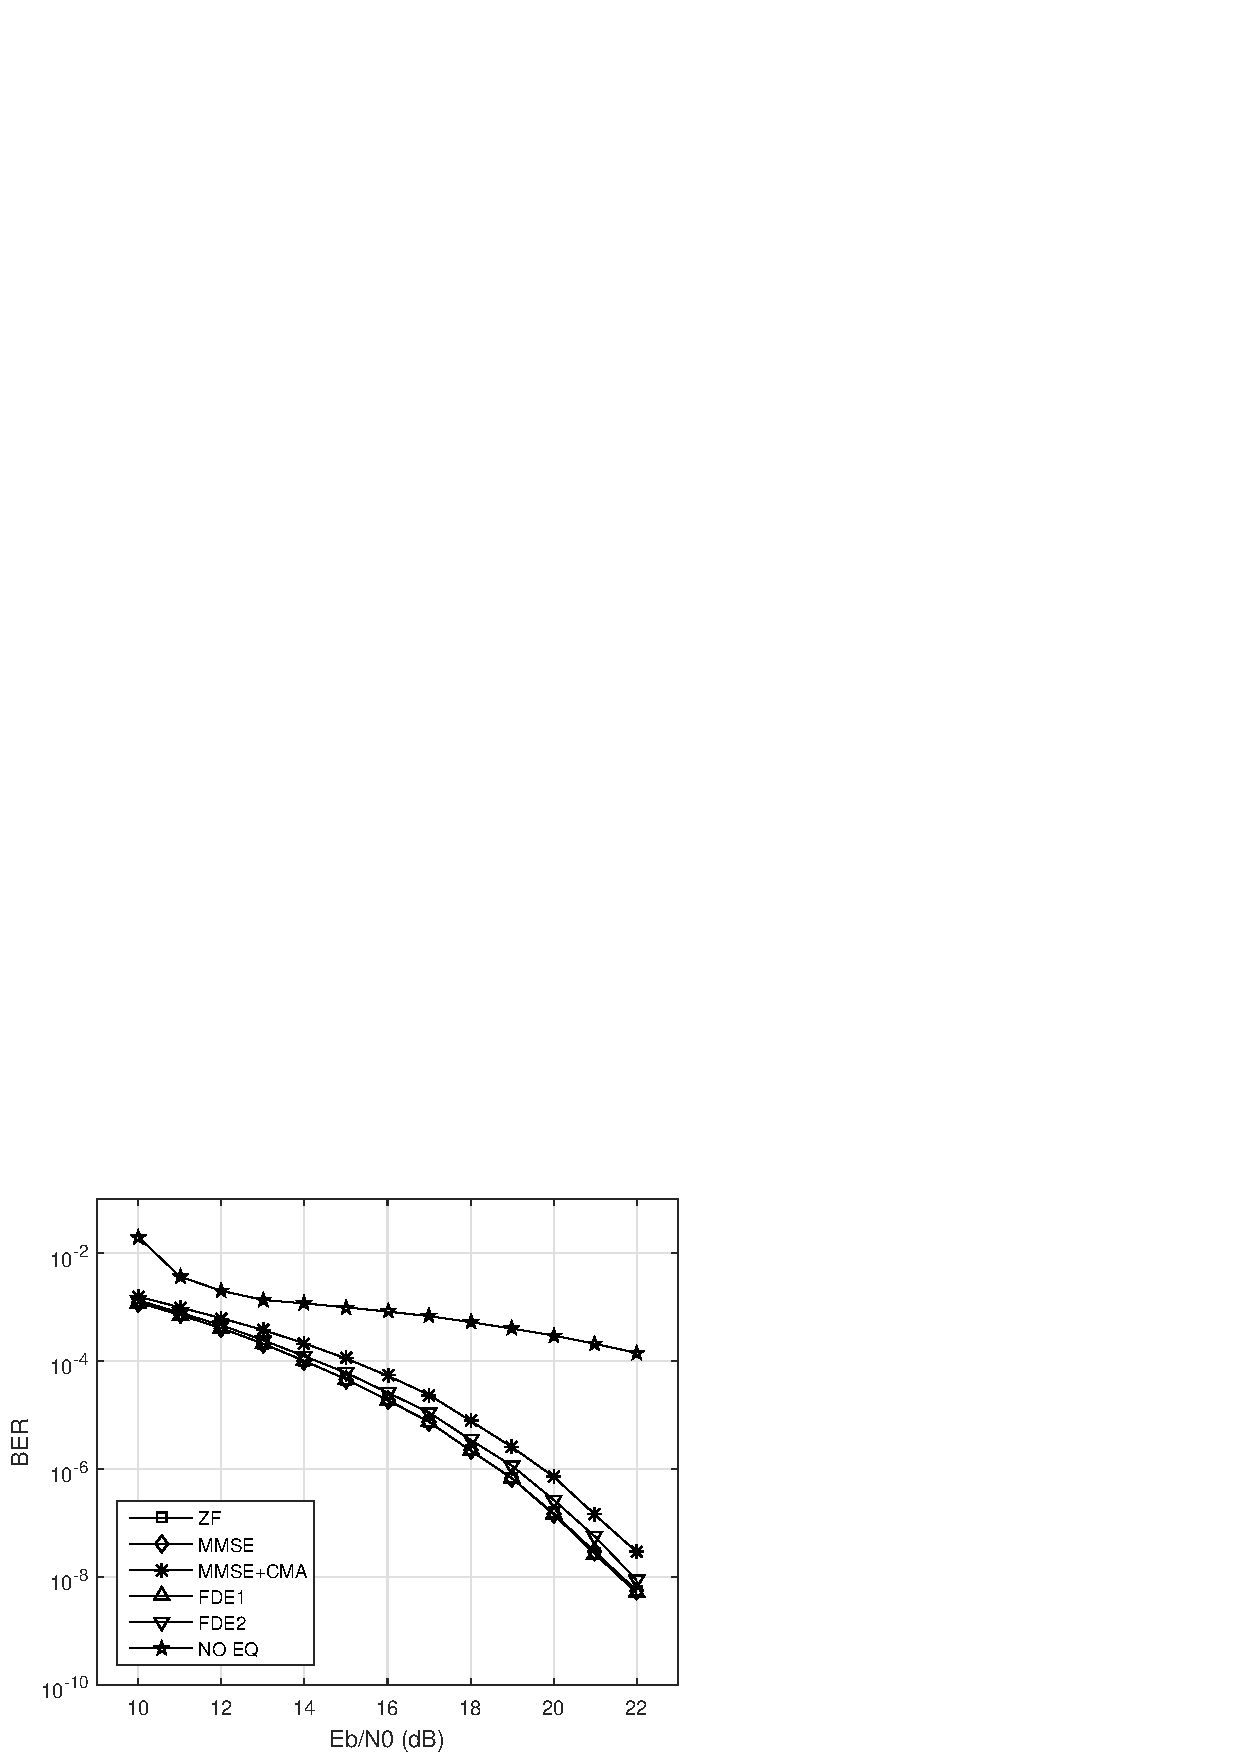
\includegraphics[width=2.5in]{figures/eq_GPUimplementation/BER1.jpg}
%			\end{minipage} 
%			& 
%			\begin{minipage}[c]{3.5in}
%				\begin{tabular}{llll}
%					\toprule
%						 		& Attenuation (dB)	& Phase ($^{\circ}$)& Delay (ns)\\ \midrule
%					Ray 1 		& 0	 				& 0 				& 0			\\
%					Ray 2 		& 1.5 				& 180 				& 50		\\
%					Ray 3 		& 20 				& 90				& 155		\\
%					\bottomrule
%				\end{tabular}
%			\end{minipage} 
%		\end{tabular}
%		\begin{tabular}{cc}
%			\begin{minipage}[c]{2.5in}
%				\centering
%				(a)
%			\end{minipage} 
%			&
%			\begin{minipage}[c]{3.5in}
%				\centering
%				(b)
%			\end{minipage} 
%		\end{tabular}
%		\\
%		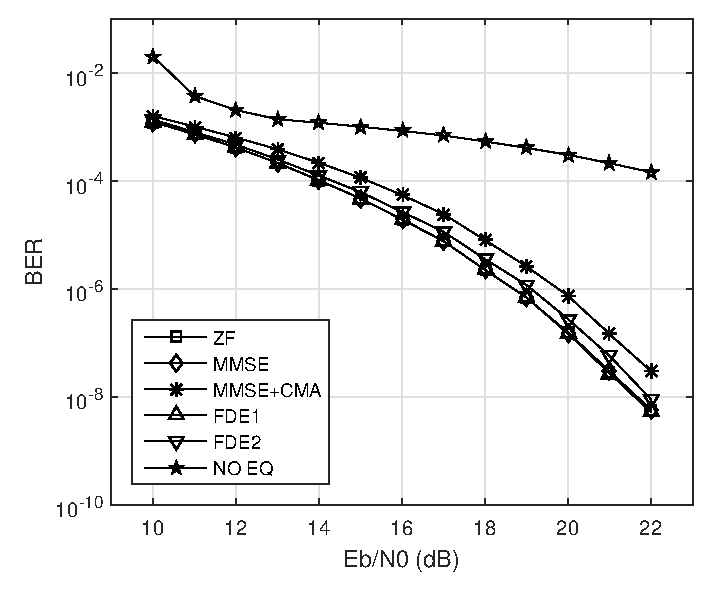
\includegraphics[width=5in]{figures/eq_GPUimplementation/BER1.eps}
%		\\
%		(c)
%	\end{center}
%	\caption{Channel 1 BER static lab test:
%	top left: a screen capture of the spectrum with averaging enabled;
%	top right: parameters for the three ray channel
%	bottom: BER curve of the five data-aided equalizers and no equalization.
%	Note that when a channel cannot lock no point is shown on the BER curve.}
%	\label{fig:BER1}
%\end{figure}
%
%\begin{figure}
%	\begin{center}
%		\begin{tabular}{cc}
%			\begin{minipage}[c]{2.5in}
%				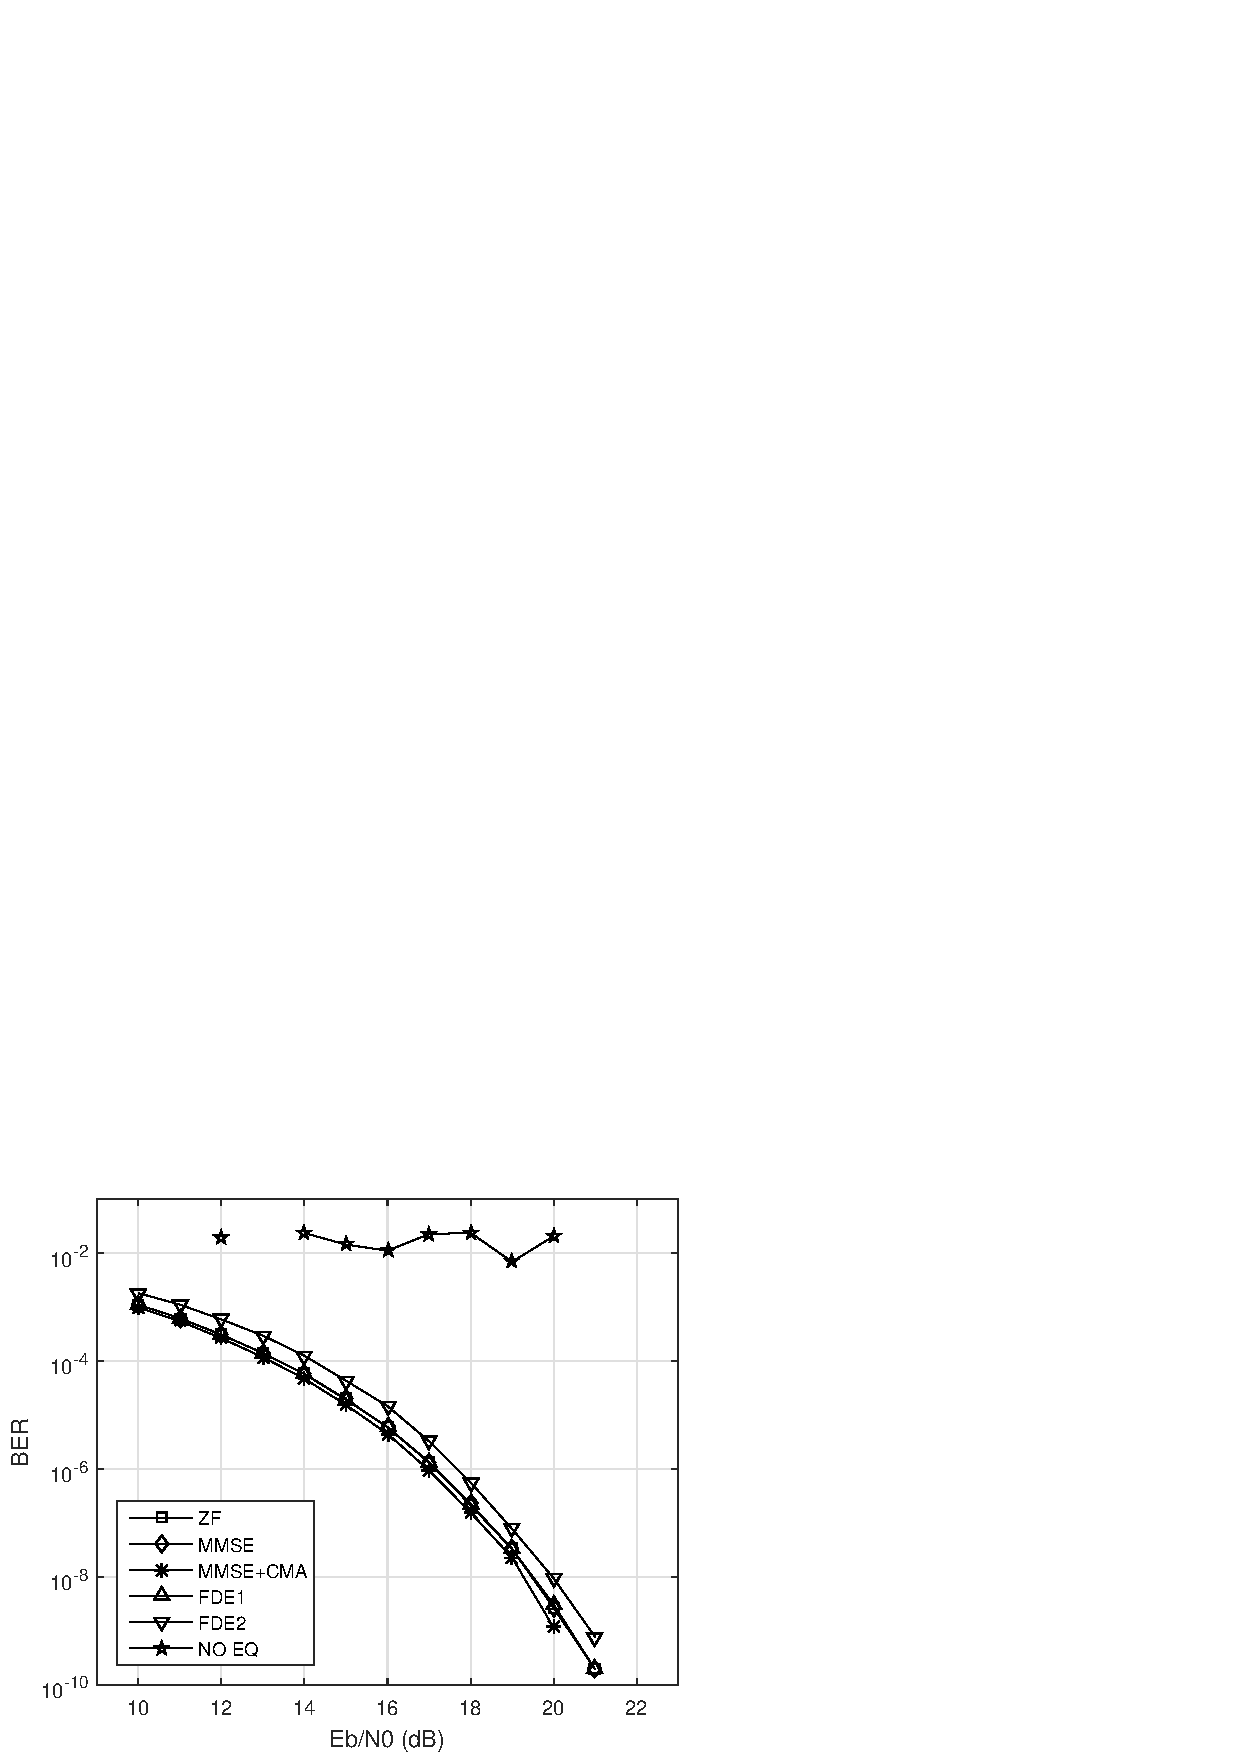
\includegraphics[width=2.5in]{figures/eq_GPUimplementation/BER2.jpg}
%			\end{minipage} 
%			& 
%			\begin{minipage}[c]{3.5in}
%				\begin{tabular}{llll}
%					\toprule
%						 		& Attenuation (dB)	& Phase ($^{\circ}$)& Delay (ns)\\ \midrule
%					Ray 1 		& 0	 				& 0 				& 0			\\
%					Ray 2 		& 1.5 				& 150 				& 50		\\
%					Ray 3 		& 20 				& 90				& 155		\\
%					\bottomrule
%				\end{tabular}
%			\end{minipage} 
%		\end{tabular}
%		\begin{tabular}{cc}
%			\begin{minipage}[c]{2.5in}
%				\centering
%				(a)
%			\end{minipage} 
%			&
%			\begin{minipage}[c]{3.5in}
%				\centering
%				(b)
%			\end{minipage} 
%		\end{tabular}
%		\\
%		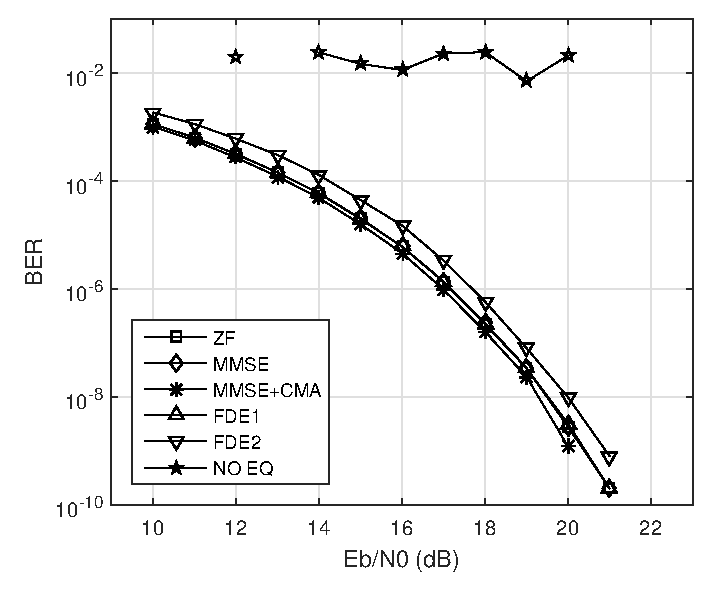
\includegraphics[width=5in]{figures/eq_GPUimplementation/BER2.eps}
%		\\
%		(c)
%	\end{center}
%	\caption{Channel 2 BER static lab test:
%	top left: a screen capture of the spectrum with averaging enabled;
%	top right: parameters for the three ray channel
%	bottom: BER curve of the five data-aided equalizers and no equalization.
%	Note that when a channel cannot lock no point is shown on the BER curve.}
%	\label{fig:BER2}
%\end{figure}
%
%\begin{figure}
%	\begin{center}
%		\begin{tabular}{cc}
%			\begin{minipage}[c]{2.5in}
%				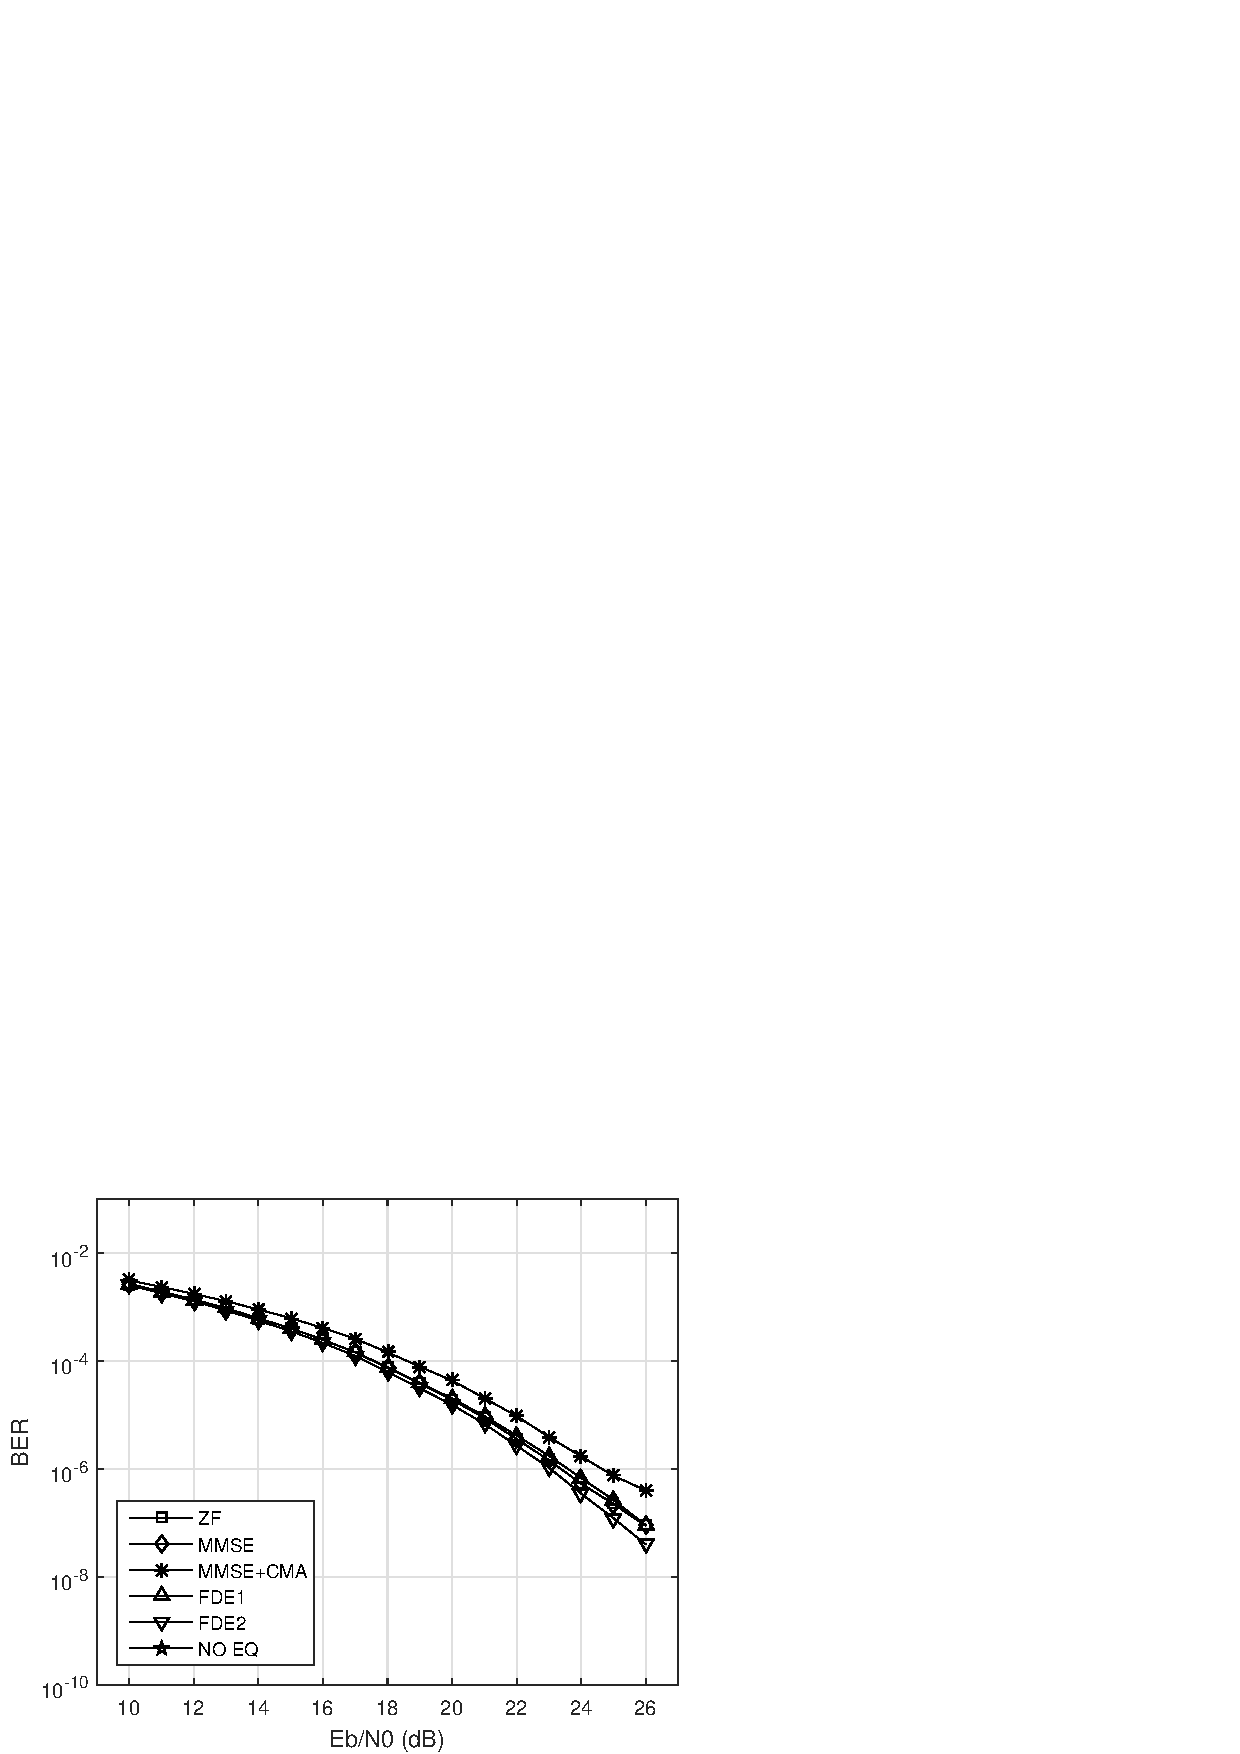
\includegraphics[width=2.5in]{figures/eq_GPUimplementation/BER3.jpg}
%			\end{minipage} 
%			& 
%			\begin{minipage}[c]{3.5in}
%				\begin{tabular}{llll}
%					\toprule
%						 		& Attenuation (dB)	& Phase ($^{\circ}$)& Delay (ns)\\ \midrule
%					Ray 1 		& 0	 				& 0 				& 0			\\
%					Ray 2 		& 1.5 				& 120 				& 50		\\
%					Ray 3 		& 20 				& 90				& 155		\\
%					\bottomrule
%				\end{tabular}
%			\end{minipage} 
%		\end{tabular}
%		\begin{tabular}{cc}
%			\begin{minipage}[c]{2.5in}
%				\centering
%				(a)
%			\end{minipage} 
%			&
%			\begin{minipage}[c]{3.5in}
%				\centering
%				(b)
%			\end{minipage} 
%		\end{tabular}
%		\\
%		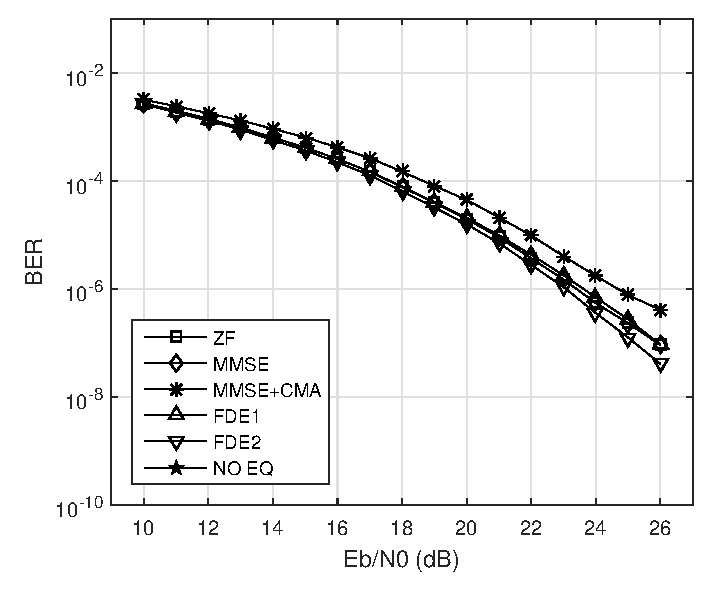
\includegraphics[width=5in]{figures/eq_GPUimplementation/BER3.eps}
%		\\
%		(c)
%	\end{center}
%	\caption{Channel 3 BER static lab test:
%	top left: a screen capture of the spectrum with averaging enabled;
%	top right: parameters for the three ray channel
%	bottom: BER curve of the five data-aided equalizers and no equalization.
%	Note that when a channel cannot lock no point is shown on the BER curve.}
%	\label{fig:BER3}
%\end{figure}

\begin{sidewaysfigure}
\begin{center}
\begin{tabular}{m{4in}m{4in}}
\multicolumn{2}{c}{
\begin{tabular}{lccc}
					\toprule
						 		& Attenuation (dB)	& Phase 					& Delay (ns)		\\ \midrule
					Ray 1 		& \hphantom{2}0.0	& $\hphantom{12}0^\circ$ 	& \hphantom{15}0	\\
					Ray 2 		& \hphantom{2}1.5 	& $180^\circ$ 				& \hphantom{1}50	\\
					Ray 3 		& 20.0 				& $\hphantom{1}90^\circ$	& 155				\\
					\bottomrule
				\end{tabular}
}
\\[54pt]
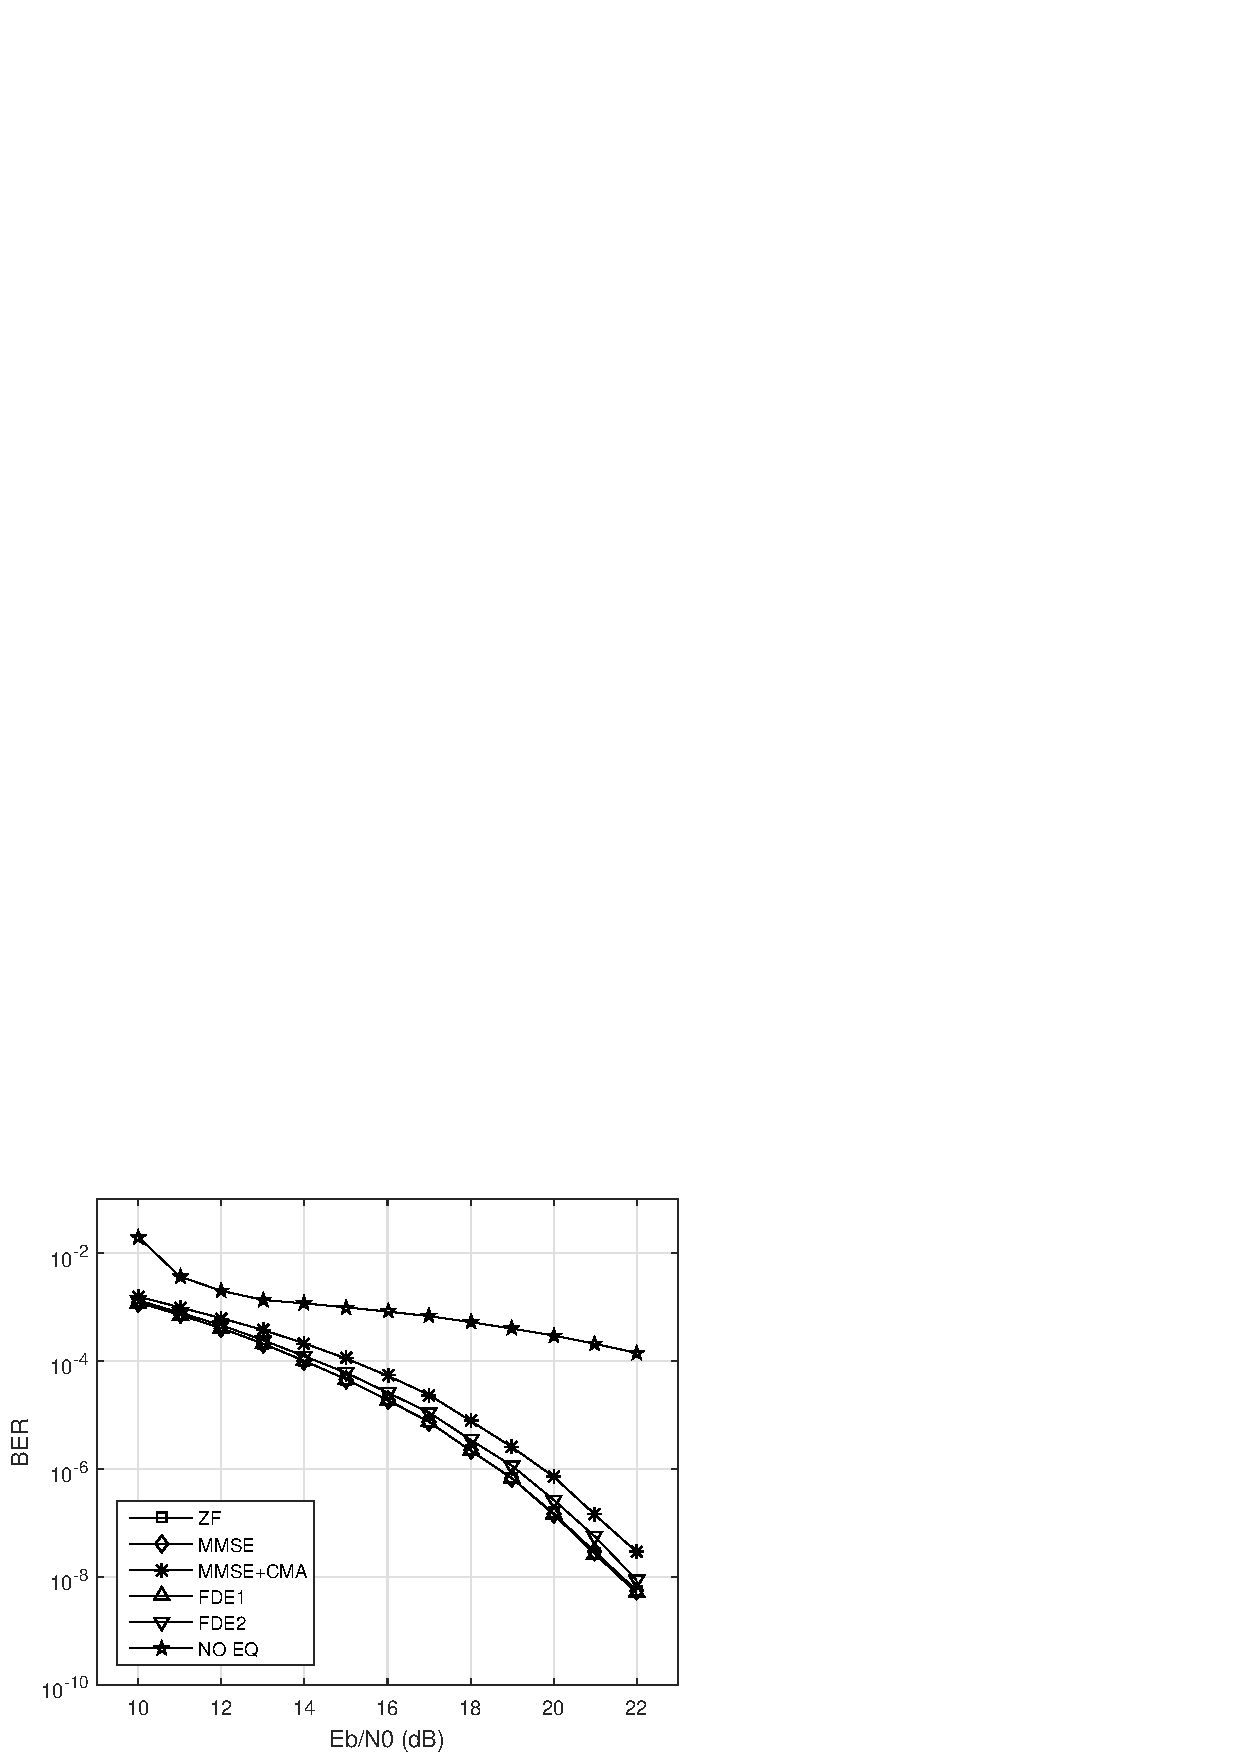
\includegraphics[width=4in]{figures/eq_GPUimplementation/BER1.jpg}
&
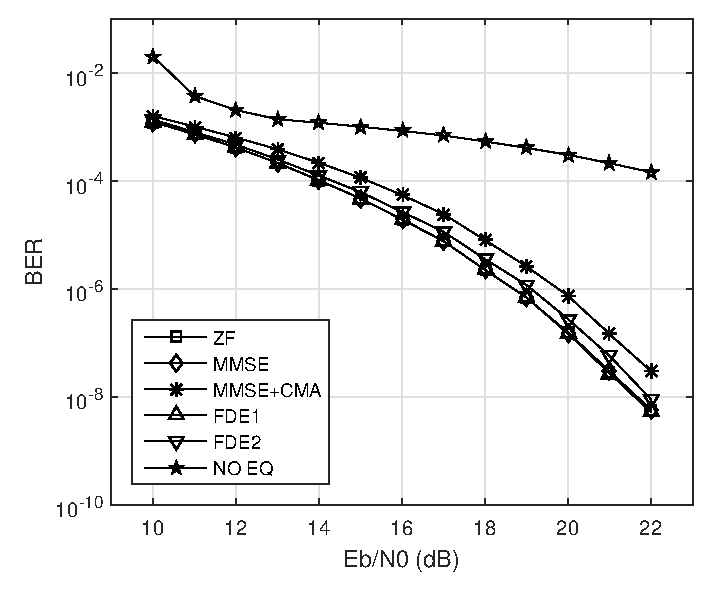
\includegraphics[width=4in]{figures/eq_GPUimplementation/BER1.eps}
\end{tabular}
\end{center}
\caption{Channel 1 BER static lab test:
(top) parameters for the three ray channel;
(bottom left) a screen capture of the spectrum with averaging enabled;
(bottom right) BER curve of the five data-aided equalizers and no equalization.}
\label{fig:BER1}
\end{sidewaysfigure}

\begin{sidewaysfigure}
\begin{center}
\begin{tabular}{m{4in}m{4in}}
\multicolumn{2}{c}{
\begin{tabular}{lccc}
					\toprule
						 		& Attenuation (dB)	& Phase 					& Delay (ns)		\\ \midrule
					Ray 1 		& \hphantom{2}0.0	& $\hphantom{12}0^\circ$ 	& \hphantom{15}0	\\
					Ray 2 		& \hphantom{2}1.5 	& $150^\circ$ 				& \hphantom{1}50	\\
					Ray 3 		& 20.0 				& $\hphantom{1}90^\circ$	& 155				\\
					\bottomrule
				\end{tabular}
}
\\[54pt]
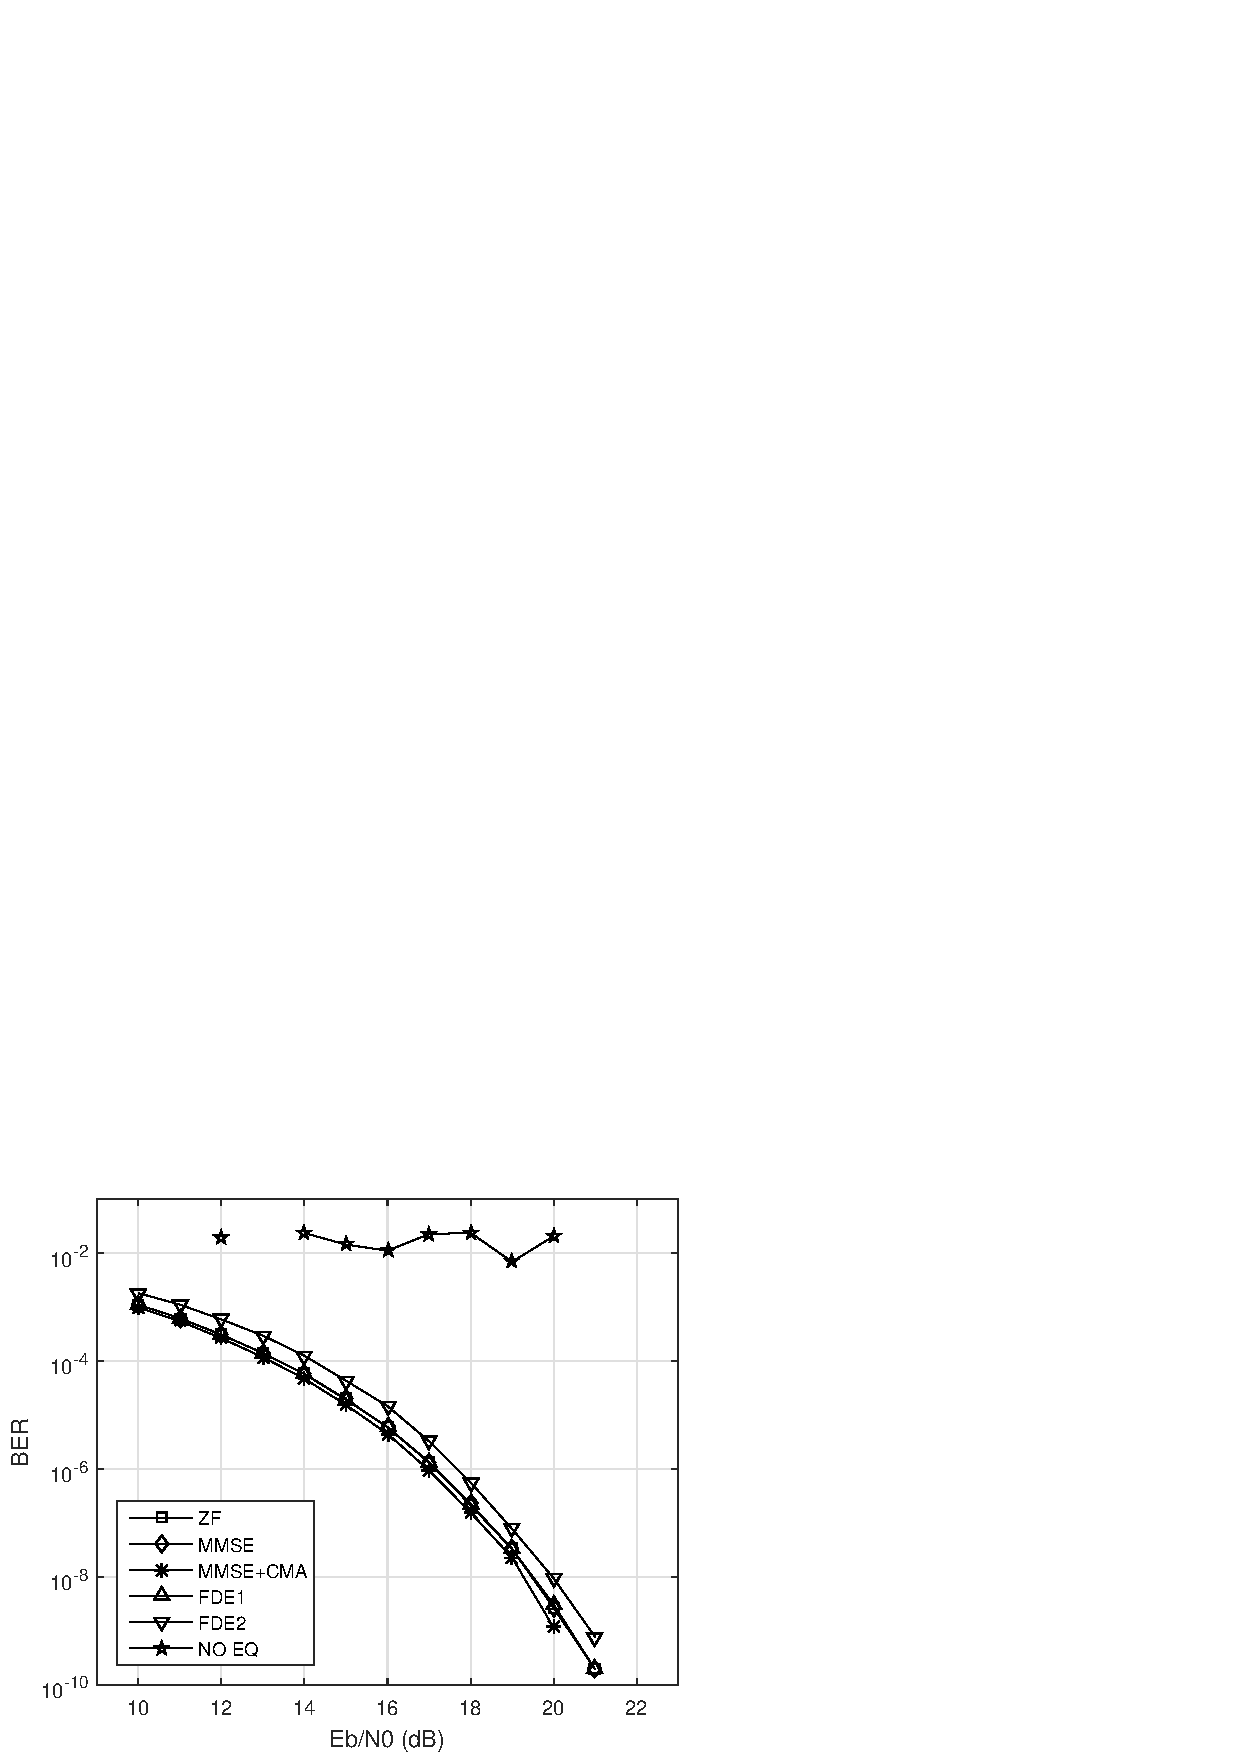
\includegraphics[width=4in]{figures/eq_GPUimplementation/BER2.jpg}
&
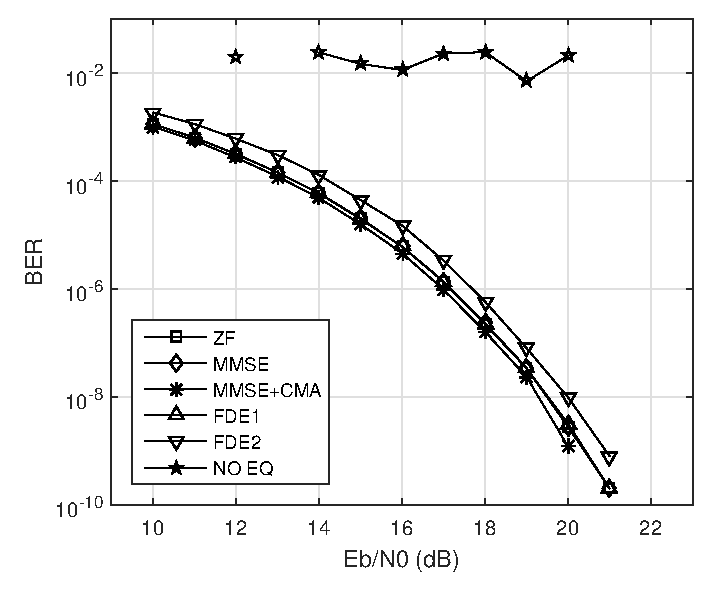
\includegraphics[width=4in]{figures/eq_GPUimplementation/BER2.eps}
\end{tabular}
\end{center}
\caption{Channel 2 BER static lab test:
(top) parameters for the three ray channel;
(bottom left) a screen capture of the spectrum with averaging enabled;
(bottom right) BER curve of the five data-aided equalizers and no equalization.
No points are shown for no equalization at some values of $E_b/N_0$ because the demodulator was unable to lock.}
\label{fig:BER2}
\end{sidewaysfigure}

\begin{sidewaysfigure}
\begin{center}
\begin{tabular}{m{4in}m{4in}}
\multicolumn{2}{c}{
\begin{tabular}{lccc}
					\toprule
						 		& Attenuation (dB)	& Phase 					& Delay (ns)		\\ \midrule
					Ray 1 		& \hphantom{2}0.0	& $\hphantom{12}0^\circ$ 	& \hphantom{15}0	\\
					Ray 2 		& \hphantom{2}1.5 	& $120^\circ$ 				& \hphantom{1}50	\\
					Ray 3 		& 20.0 				& $\hphantom{1}90^\circ$	& 155				\\
					\bottomrule
				\end{tabular}
}
\\[54pt]
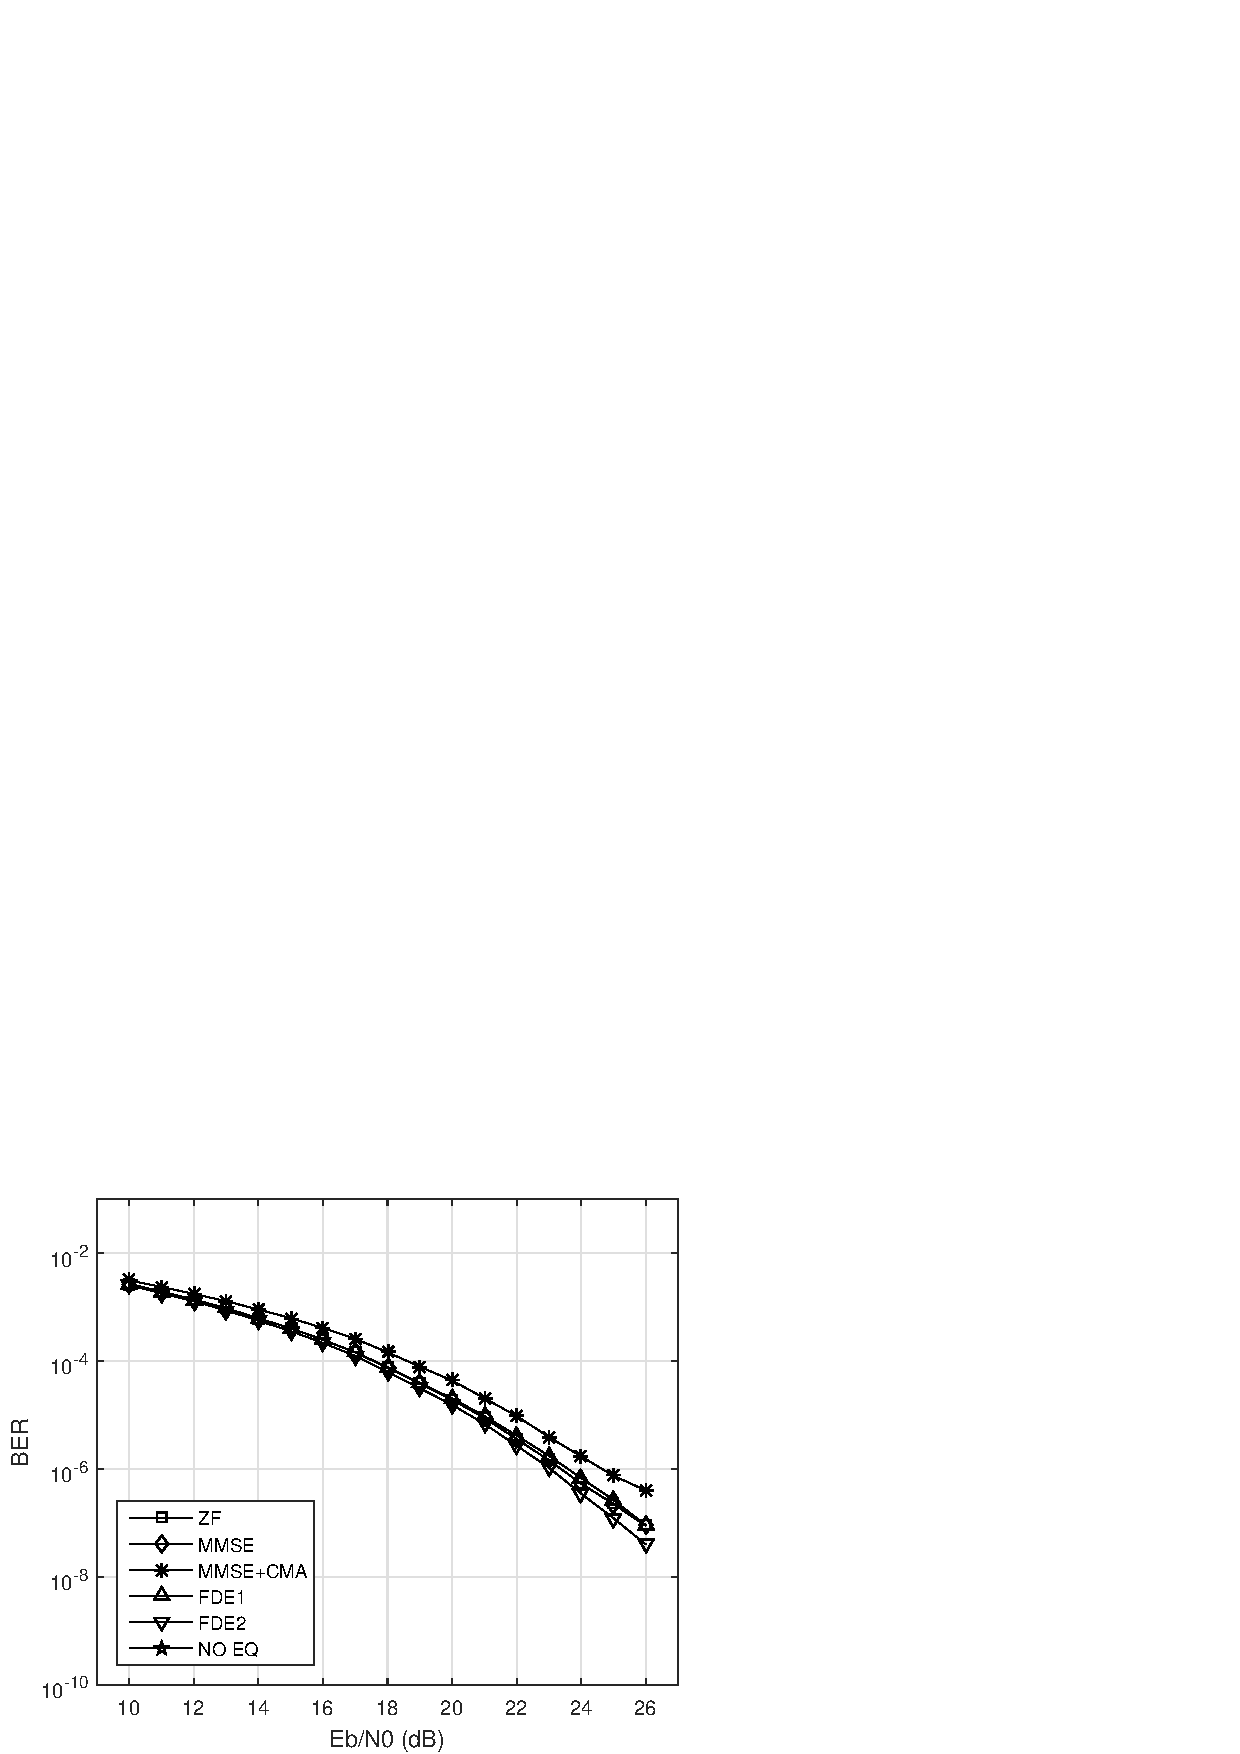
\includegraphics[width=4in]{figures/eq_GPUimplementation/BER3.jpg}
&
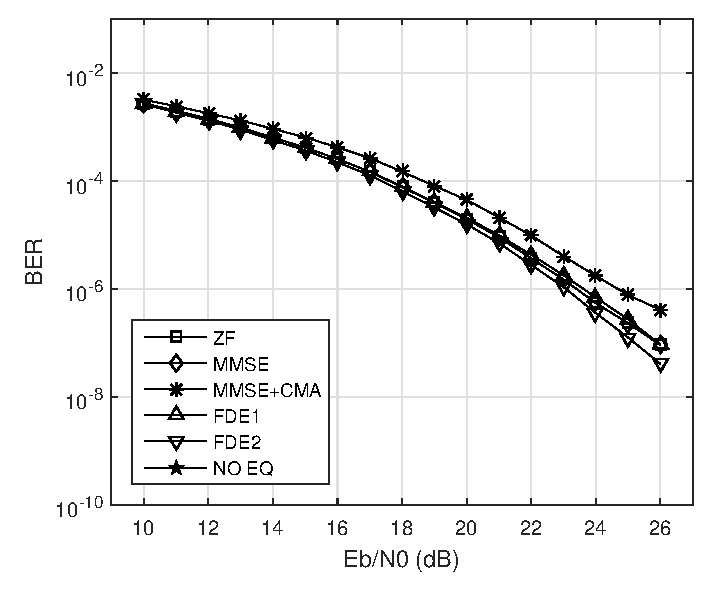
\includegraphics[width=4in]{figures/eq_GPUimplementation/BER3.eps}
\end{tabular}
\end{center}
\caption{Channel 3 BER static lab test:
(top) parameters for the three ray channel;
(bottom left) a screen capture of the spectrum with averaging enabled;
(bottom right) BER curve of the five data-aided equalizers and no equalization.
No points are shown for no equalization because the demodulator was unable to lock.}
\label{fig:BER3}
\end{sidewaysfigure}